\chapter{Findings}
Testing discovered 31 vulnerabilities and CVEs in the system, and Table \ref{table:key_findings} summarizes the key findings.

\begingroup
\centering
\setlength{\tabcolsep}{6.5pt} % Default value: 6pt
\renewcommand{\arraystretch}{1.8} % Default value: 1
\begin{longtable}{ |p{5cm}| p{10cm} |}
\caption{Severity Rankings}
    \label{table:rankings}
\hline
\rowcolor{grey!15}
\textbf{Ranking}  & \textbf{Count}\\
\hline
Critical  & 1\\
\hline
High  & 9\\
\hline
Medium  & 20\
\hline
Info  & 1\\
\hline
\hline
\textbf{Total}  & \textbf{31}\\
\hline
\end{longtable}
\endgroup
\newpage

\subsubsection{Graphs}
\begin{figure}[h!]
\centering
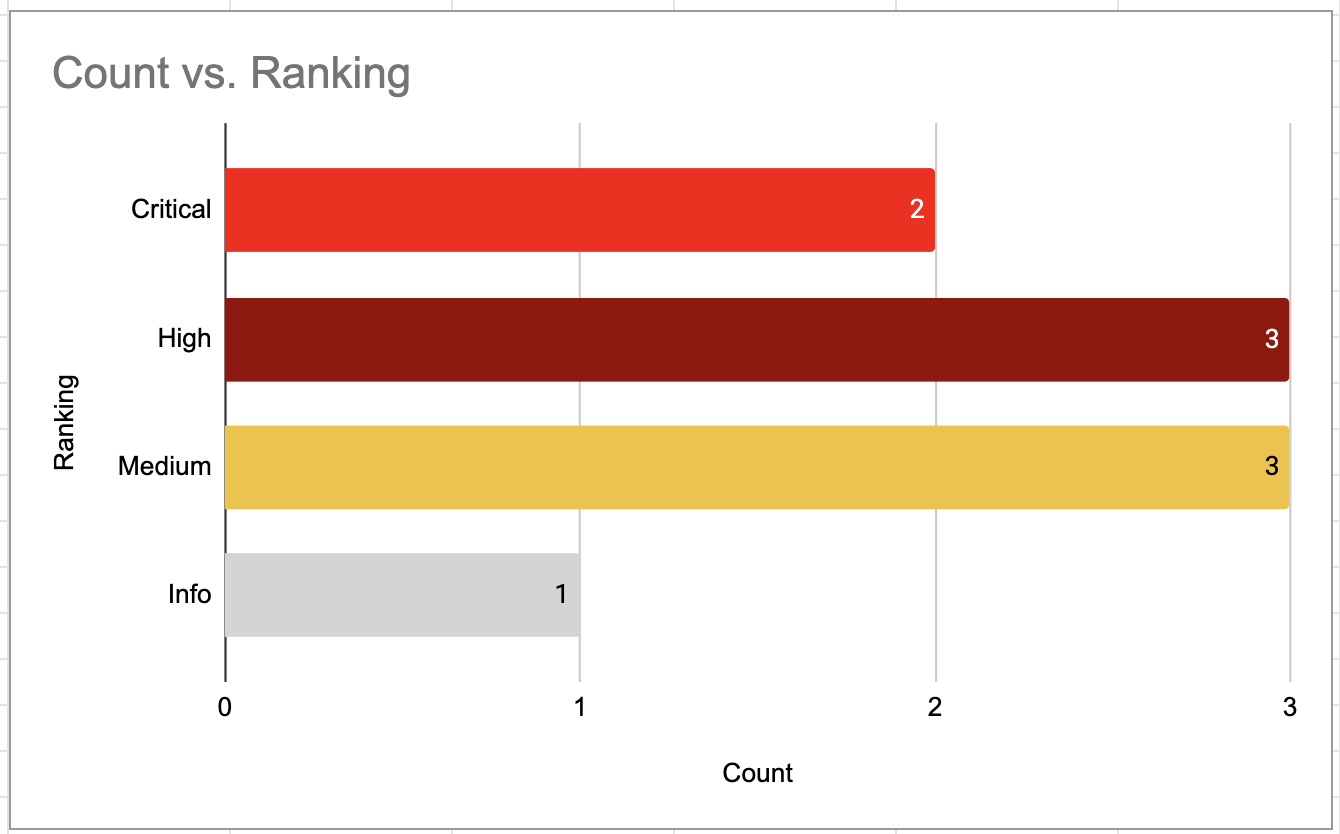
\includegraphics[width=\textwidth]{pics/rankings.png}
\caption{Distribution of risks}\label{fig:bar_risks}
\end{figure}

\begin{figure}[h!]
\centering
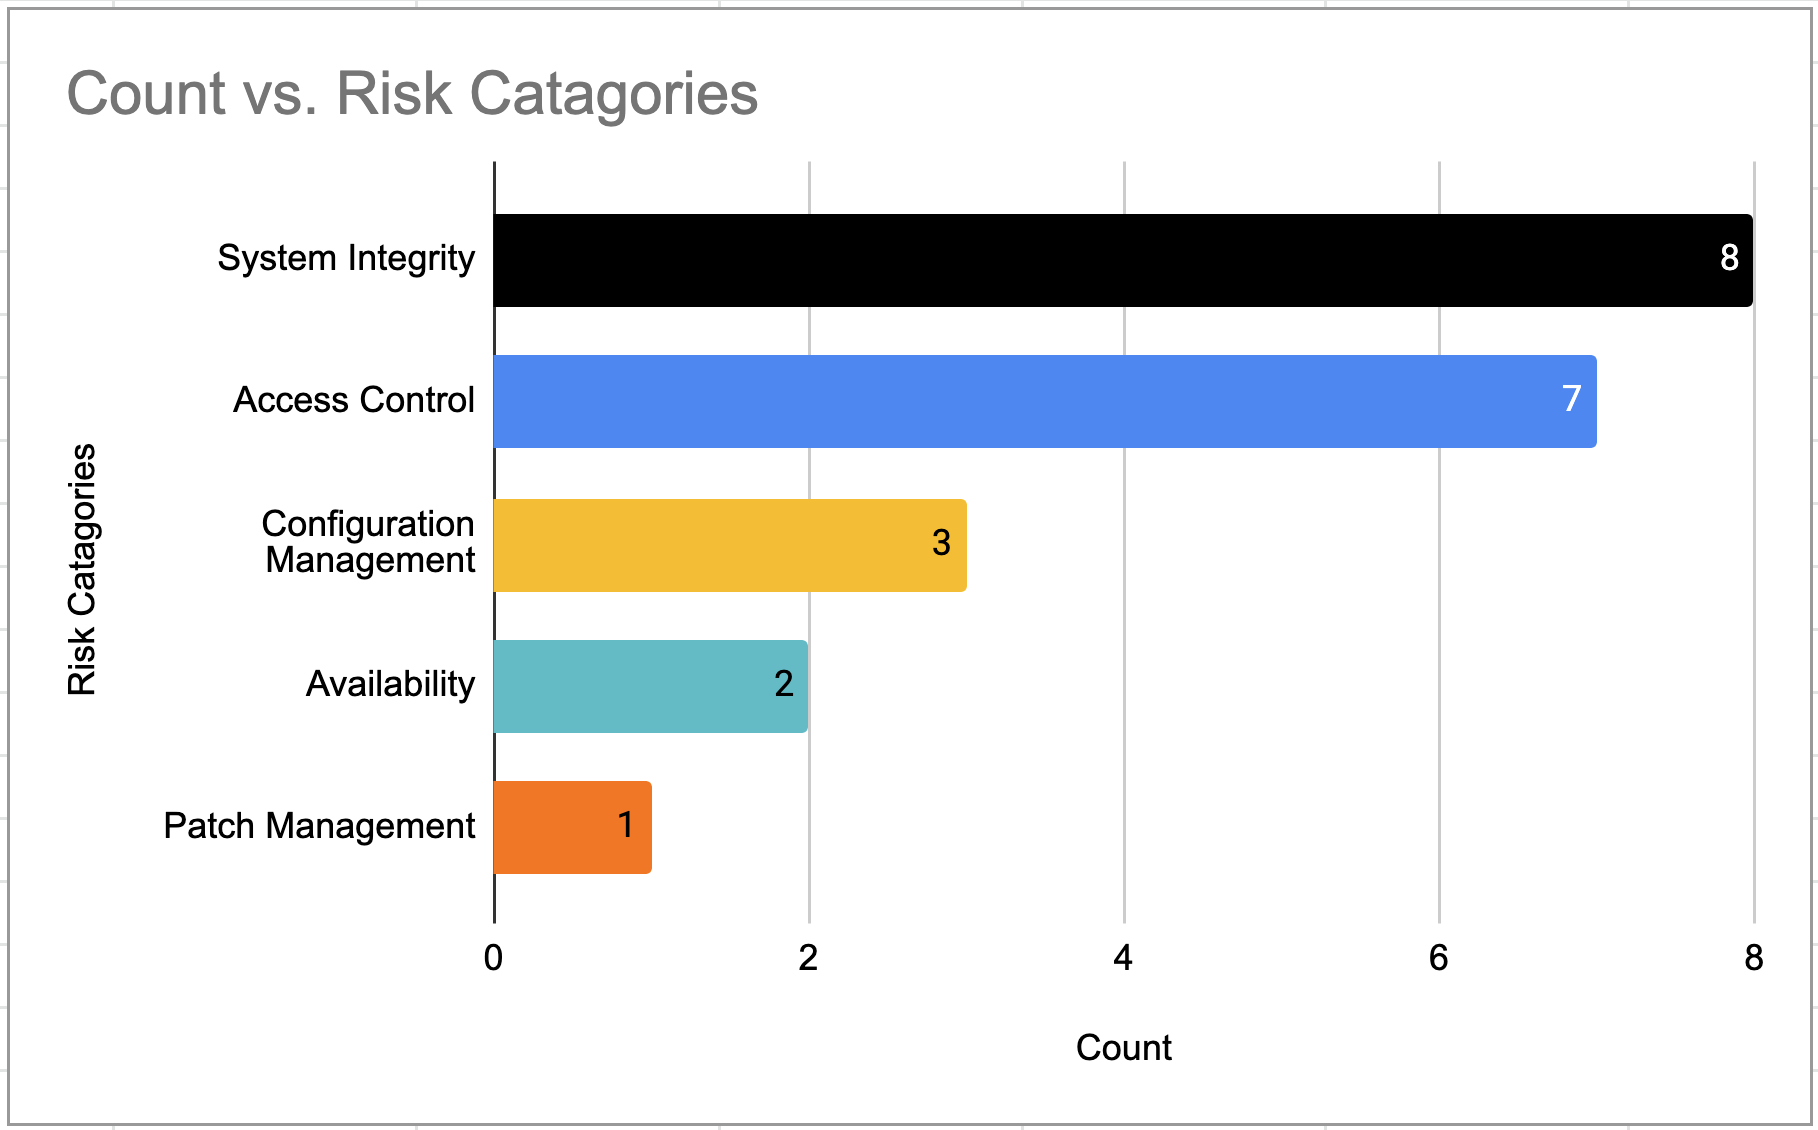
\includegraphics[width=\textwidth]{pics/risk_cat.png}
\caption{Risk Catagories Count}\label{fig:bar_risks}
\end{figure}

\section{Key Findings}
\begingroup
\centering
\setlength{\tabcolsep}{6.5pt} % Default value: 6pt
\renewcommand{\arraystretch}{1.8} % Default value: 1
\begin{longtable}{ |p{1.5cm}| p{6cm}|p{1.3cm}|p{5cm}|}
\caption{Key Findings ordered by Priority}
    \label{table:key_findings}
\hline
\rowcolor{grey!15}
\textbf{Risk}  & \textbf{Finding}& \textbf{Count}& \textbf{Solution}\\
\hline
\cellcolor{red!95} Critical  & Externally exposed Network Resources, i.e., databases, FTP, DNS servers. Information theft and DoS attack are highly likely.
\newline (Configuration Management). & 1 & Ports 21, 3306, and 5432 should be closed from the public internet as they are not necessary to be open for running the CMS. CDN should be used to relieve the load on the servers.
\\
\hline
\cellcolor{red!70} High  & Insecure database versions  containing multiple CVEs. This can lead to personal data theft.
\newline (Patch Management).& 7 & The vulnerable versions of database must be updated to a secure one. In addition, regular security automatic scans with dynamic and static application testing should be carried out.
\\
\hline
\cellcolor{red!70} High  & Malicious Code injection possible(XSS, CSRF forgery) 
\newline (System Integrity)& 2 & The HTML inputs should be sanitized, set Content-security policy header, and CSRF tokens \citep[p.~75]{xss_crsf}.
\\
\hline
\cellcolor{yellow!95} Medium  & Ip spoofing, DNS server spoofing and Cache Poisoning possible.
\newline (System Integrity) .& 2 & Implement DNSSEC to protect the integrity of the server and turn off DNS recursion in the Bind server. \citep[p.~38]{guo2006spoof}
\\
\hline
\cellcolor{yellow!95} Medium  & Server and application version is public 
\newline(Configuration Management).& 2 & Do not make server and application versions public information.
\\
\hline
\cellcolor{yellow!95} Medium  & DNS server is outdated, can cause an outage of the service because of present vulnerabilities.
\newline (Patch management).& 16 & Update DNS bind to v9.18.12.
\\
\hline
\cellcolor{grey!55} Info  & Application discloses system information
\newline (Configuration Management).& 1 & Only generic errors should be outputted, and application information in error should be removed.
\\
\hline
\end{longtable}
\endgroup
\newpage